% Created 2023-11-04 sáb 12:57
% Intended LaTeX compiler: pdflatex
\documentclass[11pt]{article}
\usepackage[utf8]{inputenc}
\usepackage[T1]{fontenc}
\usepackage{graphicx}
\usepackage{grffile}
\usepackage{longtable}
\usepackage{wrapfig}
\usepackage{rotating}
\usepackage[normalem]{ulem}
\usepackage{amsmath}
\usepackage{textcomp}
\usepackage{amssymb}
\usepackage{capt-of}
\usepackage{hyperref}
\usepackage{../../modern}
\bibliography{./fuentes.bib}
\raggedbottom
\setcounter{secnumdepth}{2}
\author{Luis Eduardo Galindo Amaya (1274895)}
\date{jueves, 02 noviembre 2023}
\title{Práctica No. 4 Taller}
\hypersetup{
 pdfauthor={Luis Eduardo Galindo Amaya (1274895)},
 pdftitle={Práctica No. 4 Taller},
 pdfkeywords={},
 pdfsubject={},
 pdfcreator={Emacs 27.1 (Org mode 9.3)}, 
 pdflang={Spanish}}
\begin{document}

\modentitlepage{../../images/escudo-uabc-2022-1-tinta-pos.png}
\datasection{Individual}

\tableofcontents
\pagebreak

\section{Modelos de representación de conocimiento}
\label{sec:org8bbcff0}
Deacuerdo a \autocite{prasad2012hybrid} algunos de los metodos
mas coumnes para representar conocimiento son:

\subsection{Red Bayesiana}
\label{sec:orgf6e561a}
\autocite{Sucar} Las redes bayesianas modelan un fenómeno
mediante un conjunto de variables y las relaciones de dependencia
entre ellas. Dado este modelo, se puede hacer inferencia bayesiana; es
decir, estimar la probabilidad posterior de las variables no
conocidas, en base a las variables conocidas.

\begin{figure}[htbp]
\centering
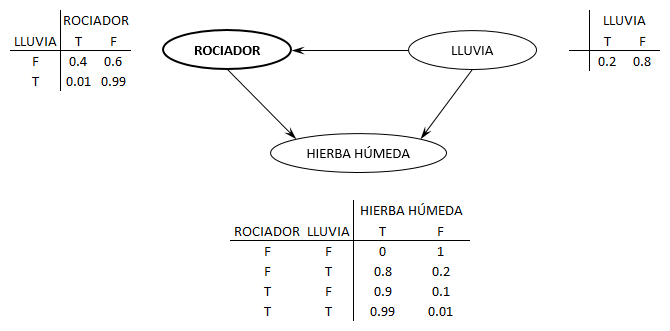
\includegraphics[width=12cm]{img/Red_Bayesiana_Simple.png}
\caption{Ejemplo de una red bayesiana simple.}
\end{figure}

\subsection{Facts and Production Rules}
\label{sec:org0a8a0fb}
\autocite{expert_systems} Una regla de producción, o simplemente
una regla, consta de una parte SI (una condición o premisa) y una
parte ENTONCES (una acción o conclusión). SI condición ENTONCES acción 
(conclusión). La facilidad de explicación explica cómo el sistema
llegó a la recomendación. Dependiendo de la herramienta utilizada para 
implementar el sistema experto, la explicación puede estar en lenguaje
natural o simplemente ser una lista de números de reglas.

\subsection{Redes semánticas}
\label{sec:org6a4a179}
\autocite{Sowa_1993} Una red semántica es una estructura de grafo
para representar conocimiento en patrones de nodos interconectados y
arcos. 

\begin{figure}[htbp]
\centering
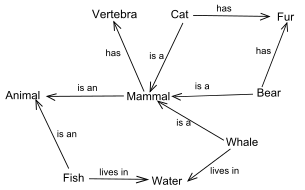
\includegraphics[width=10cm]{img/Semantic_Net.png}
\caption{Ejemplo de una red semántica}
\end{figure}

\subsection{Dependencia Conceptual}
\label{sec:org55ce958}
\autocite{Raghavavaiah} Esta representación se utiliza en el
procesamiento de lenguaje natural con el fin de representar el
significado de las oraciones de tal manera que se puedan realizar
inferencias a partir de ellas. Es independiente del idioma en el que
originalmente se expresaron las oraciones. Las representaciones de CD
(Conceptual Dependency) de una oración se construyen a partir de
primitivas que no son palabras del idioma, sino conceptuales. Estas
primitivas se combinan para formar los significados de las palabras. 

\subsection{Frames}
\label{sec:org6fd7fab}
\autocite{Minsky_1974} Un 'frame' es una estructura de datos para
representar una situación estereotipada, como estar en un cierto tipo
de sala de estar o asistir a una fiesta infantil. A cada marco se le
adjuntan varios tipos de información. Alguna de esta información trata
sobre cómo usar el marco. Otra parte se refiere a lo que se puede
esperar que suceda a continuación. También se incluye información
sobre qué hacer si las expectativas no se confirman. 

\subsection{Guiones}
\label{sec:orgffe7140}
\autocite{Schank1975ScriptsPA} Un guion es una secuencia
predefinida y estereotipada de acciones que define una situación muy
conocida. En efecto, un guion es una historia bastante aburrida. Los
guiones permiten hacer referencia a objetos dentro de ellos como si
estos objetos hubieran sido mencionados previamente. 

\subsection{Sistemas hibridos}
\label{sec:orgdd80c06}
\autocite{prasad2012hybrid} Un sistema de conocimiento híbrido es
una implementación de un formalismo de conocimiento híbrido que consta
de dos o más subformalismos diferentes. 


\section{Definición matemática de redes semánticas}
\label{sec:orgab8d76a}
\autocite{Hernandez_Karelin_Tarasenko_2014} Dado un fragmento de
la realidad y un fenómeno físico de ingeniería u otro tipo de problema
que se deba modelar, podemos proponer lo siguiente: si \textbf{P} es un
conjunto de oraciones en lenguaje natural que describe dicho fenómeno
y si el conjunto correspondiente \textbf{K} de fórmulas bien formadas derivadas
de \textbf{P}, como resultado de la transcripción del lenguaje natural,
utilizando un lenguaje formal intermedio como el cálculo de predicados
de primer orden, entonces existe una red semántica de \textbf{P} que
corresponde al problema en cuestión.  

\section{Red Semantica de conocimiento personal}
\label{sec:org94849d4}
\begin{figure}[htbp]
\centering
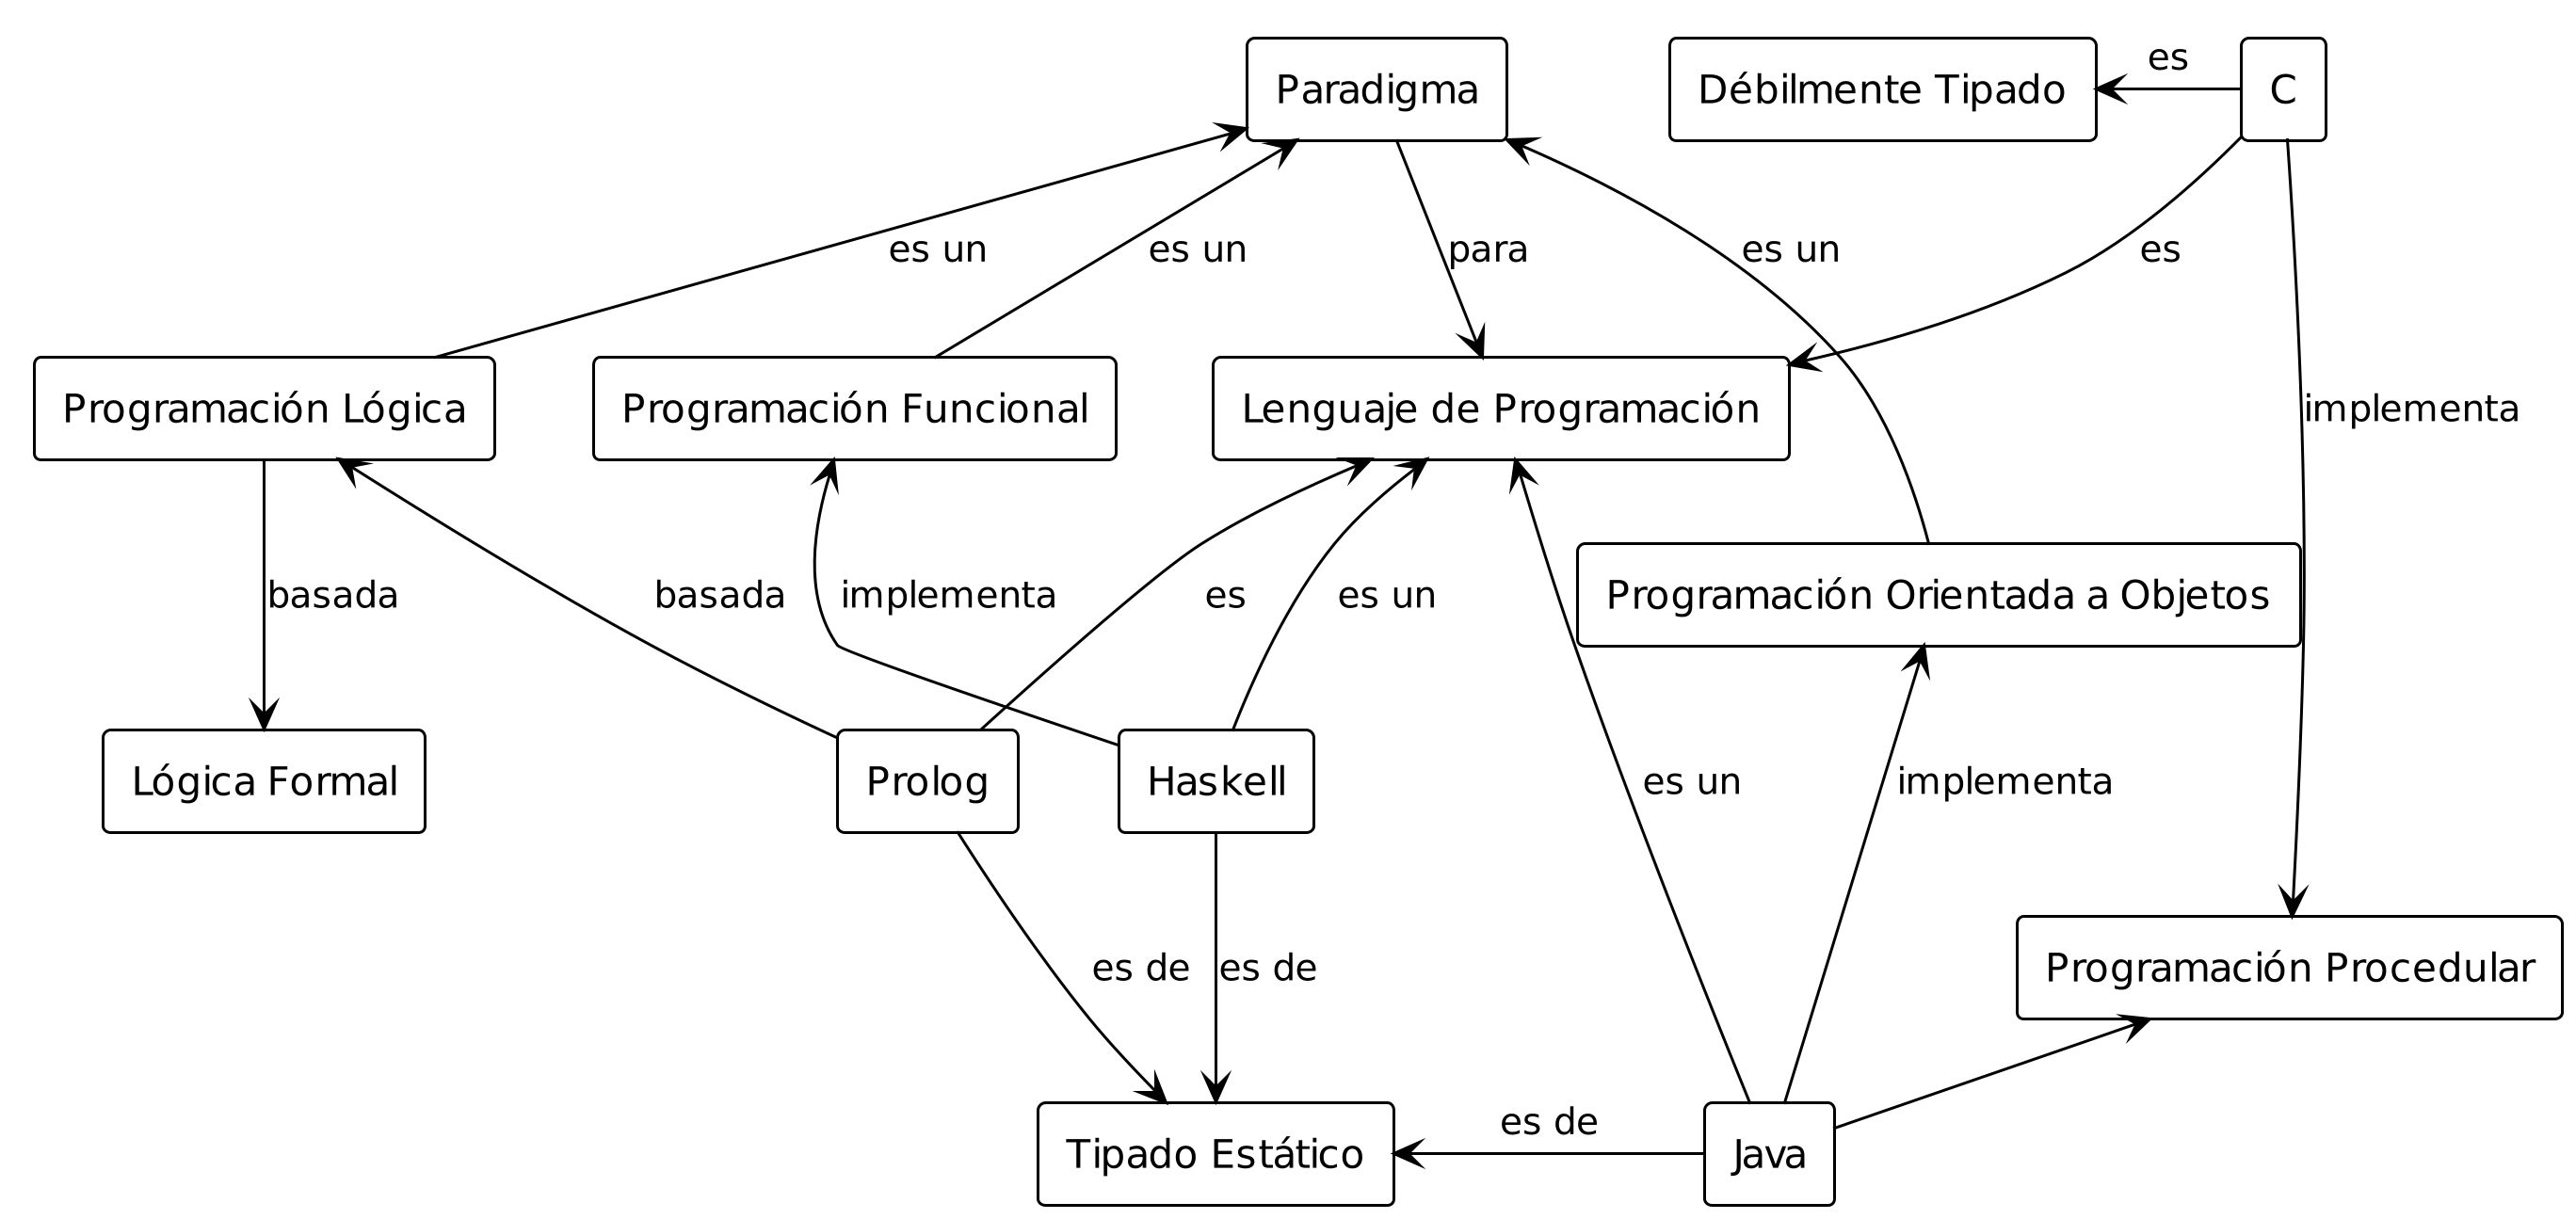
\includegraphics[width=.9\linewidth]{./img/test.png}
\caption{Red semántica de 'Lenguajes y Paradigmas'.}
\end{figure}

\section{Conclusión}
\label{sec:org3792f87}
A lo largo de la practica aprendí como diversos tipos de
representaciones permiten que las computadoras puedan aprender sobre
conceptos o ideas de maneras similares a como las entendemos los
humanos, la representación del conocimiento puede ser utilizada de
manera mas eficiente si la representación permite analizar el dominio
del problema de manera mas eficiente.

\section{Referencias}
\label{sec:org3b307ec}
\printbibliography[heading=none]
\end{document}
